\section{Anexos}

\subsection{Flujo de trabajo en BASH}

Hemos planteado el flujo de BASH de la siguiente manera:
Tendremos un archivo principal \textit{launch.sh} que se ejecuta desde la consola pasándole como parámetro la ruta de la carpeta donde se guardarán los resultados. Este comprobará si están instalados los paquetes necesarios para la ejecución del código. Si estos están instalados en la carpeta \textit{software/deps-r} (Porque ya se haya ejecutado previamente el archivo \textit{setup.sh}), se ejecutará directamente el archivo \textit{human-covid-network.R}. La ejecución del archivo mostrará resultados numéricos, como el diámetro de la red, por pantalla y generará gráficos en formato PNG y PDF. 

\begin{center}

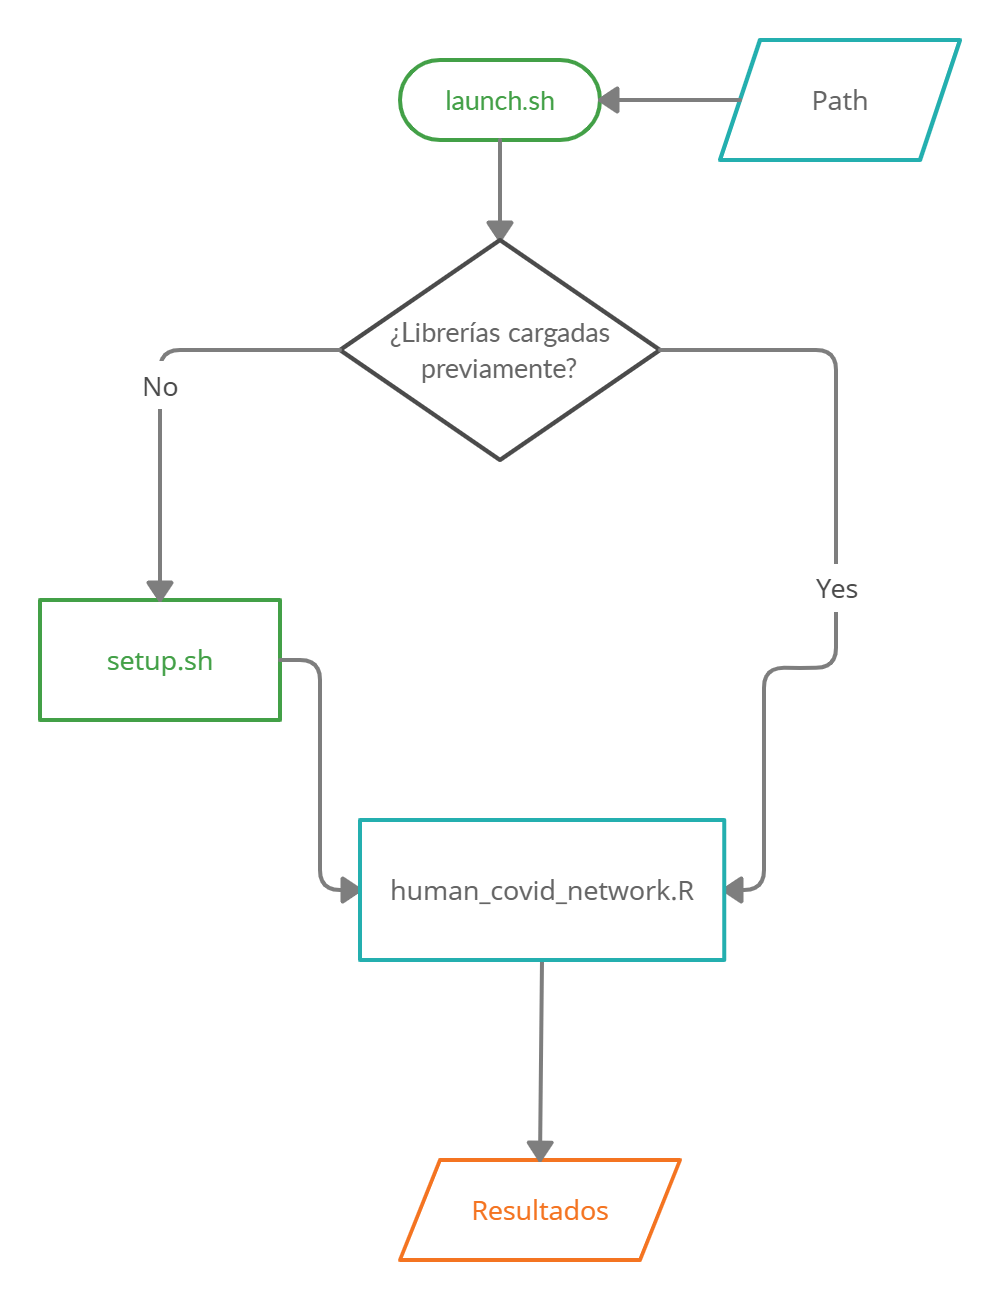
\includegraphics[width=90mm,scale=1]{report/figures/flujo.PNG}

\end{center}

\subsection{Ejecución}
Es necesaria la ejecución desde un terminal Linux, ya que algunas de las librería que se han utilizado para realizar este trabajo solo pueden instalarse desde ahí.
Además, deberemos disponer de la versión 4.0 o superior de R para poder acceder a la versión más actualizada de STRINGdb(Si se usa una versión anterior se generaran resultados distintos a los expuestos en esta memoria.
